\section{SwipeVR  Design Concepts }
Our design efforts focused on balancing three of the above factors: input speed, learning time, and physical size.
Our thinking was particularly influenced by the interaction design of cell phones that use T9 input, which relies on a database of words to disambiguate cell phone keypad keystrokes that are associated with more than one letter.
If we could design an input device that combined the best of the standard keyboard (fast text input, familiar layout) and the 12-key cell phone keypad (small size), we would have a device that could be used in off-the-desktop situations, potentially for extended typing tasks, with little degradation in performance. 

\subsection{Key Grouping}
Even with relative finger tracking, typing in virtual reality still possesses the challenge that dragging to a specific key is slow and cumbersome given the limited screen space available for a mobile phone.
As users pick up the pace they are typing, their accuracy decreases for dragging precisely to individual letters.
To sustain the speed that they are typing in for each swipe requires considerable motion to complete with accuracy.
Thus, taking inspiration from traditional T9 keyboard widely used in feature phones, we arrive at a similar design choice of batching keys together to form sections that will register for all the keys in the section.
We group keys for efficiency(Hick's law)~\cite{card1983psychology}.

The advantages of such batched keys are two-fold.
Firstly, by batching some keys together, the user no longer need to be that precise in his dragging.
As long as he reaches within the proximity of the target letter, the whole region will register.
Secondly, by batching the keys together, we allow users to simply drag to direction of the key instead of having to take effort to get to the target letter, which drastically reduce the work a user has to do in a single swipe.

\subsection{Relative Positioning}
Traditional mobile keyboard requires users to tap on the key precisely to enter an individual letter.
This method falls prey to specifically to the problem described above: users cannot tap on the individual keys accurate enough because they cannot see their finger relative to the touch screen of the mobile phone in a virtual environment.
Thus, we seek to use relative finger tracking to control a virtual cursor to solve the problem that users cannot see their hands.
Instead of having to be very precise about his finger positions, we instead rely on finger swiping or dragging to control a cursor in virtual reality.
Thus, users no longer need to consider the initial position of his finger because only the change in his finger position will be accounted for. 
Relative movement, instead of absolute movements, have also been found to be beneficial in reducing fatigue~\cite{Hincapie-Ramos:2014:CEM:2556288.2557130} so the user can start the interaction from their current position.

\subsection{Proprioception}
The most prominent problem for a traditional keyboard in a virtual environment setting is that the user cannot see the actual keyboard that he or she is using or his own finger.
Even though there can be realistic representation of the keyboard and his fingers in VR, users still suffer from not being able to see some part of his own body.
The solution to such visual segmentation is not apparent, for whole body tracking in VR is not yet available.

Despite the difficulties for the users to physically locate their finger outside of the virtual environment in order to interact with the keyboard on a mobile phone, the users are not completely helpless from their previous typing experience.
To start with, the users have muscle memory from typing on traditional mobile keyboards. With this previous experience, the user remembers, although imprecise, the location of letters if the layout of the keyboard is the same as what they are used to.

Studies show that users possesses approximate knowledge of where their fingers are on screen thanks to proprioception \cite{boff1986handbook}.
Thus, to leverage these previous knowledge of the users and address the problem that the users cannot physically see their fingers, we center our designs around two key features that we believe can help them adjust to typing in virtual reality: relative finger tracking, and batched keys.

\begin{figure*}
  \centering
  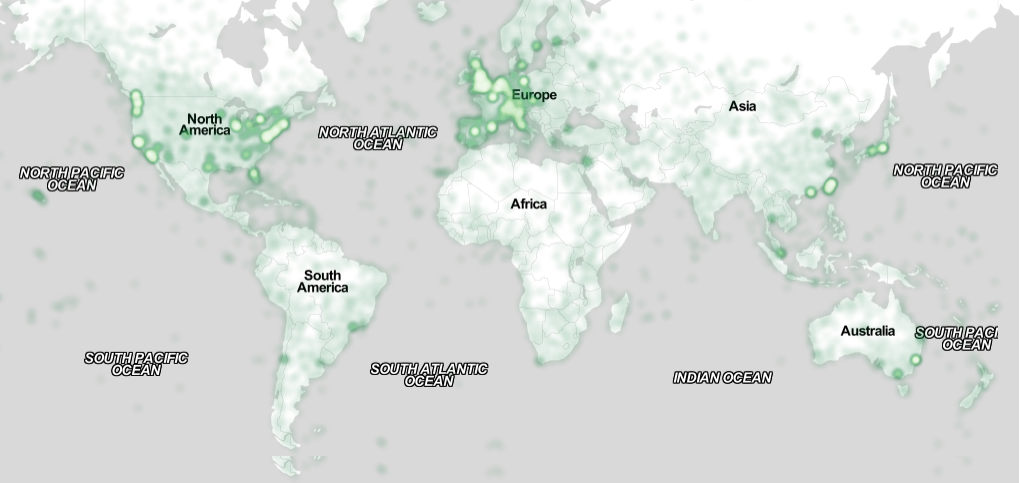
\includegraphics[width=1.75\columnwidth]{figures/map}
  \caption{Example of the system.  When the user want to type .}
  ~\label{fig:example}
\end{figure*}



\begin{figure}
\centering

  \begin{tikzpicture}

  \def \n {5}
  \def \radius {3cm}
  \def \margin {8} % margin in angles, depends on the radius

  \foreach \s in {1,...,\n}
  {
    \node[draw, circle] at ({360/\n * (\s - 1)}:\radius) {$\s$};
    \draw[->, >=latex] ({360/\n * (\s - 1)+\margin}:\radius) 
      arc ({360/\n * (\s - 1)+\margin}:{360/\n * (\s)-\margin}:\radius);
  	}
	\end{tikzpicture}

	\caption{
    Controller\\
	Intent Detection Classifier\\
    triager \\
	|swipe          |                |\\
    ngram           deterministic     \\
    selection        letter           \\
}~\label{fig:systemFlowchart}
\end{figure}

